In task 0 we want to discretize the dynamics, write the discrete-time state-space equations and code the
dynamics function.

\section{State space and control inputs}
The system can be modeled as a planar quadrotor with a downward pendulum attached
at its center of mass, representing the load,
as shown in Figure \ref{fig:quadrotor}.

\begin{figure}[htp]
\centering
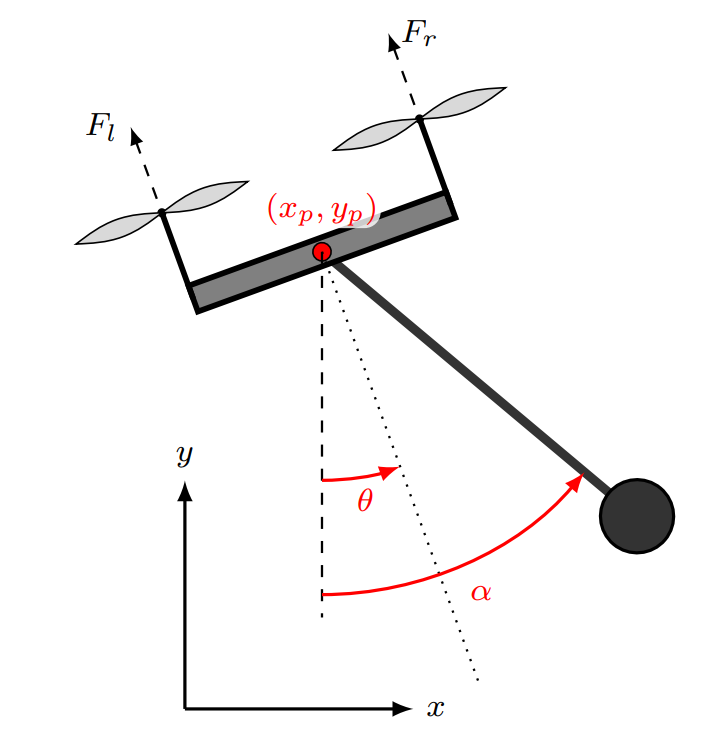
\includegraphics[width=0.5\textwidth]{pictures/quadrotor}
\caption{Model of a planar quadrotor with a suspended load}
\label{fig:quadrotor}
\end{figure}

The state space consist in \[ x = [x_p, y_p, \alpha, \theta, v_x, v_y, \omega_\alpha, \omega_\theta]^T\] where $(x_p, y_p) \in \mathbb{R}^2$ represent the position of the center of mass, $\theta$ the roll angle of the quadrotor, $\alpha$ the angle of the pendulum with respect to the inertial frame, $(v_x, v_y)$ the velocity of the center of mass, $\omega_\alpha$ and $\omega_\theta$ angular rate of changes associated to $\alpha$ and $\theta$, respectively.

The input is \[u = [F_s, F_d]^T\] where \[\begin{cases}F_s = F_l + F_r \\ F_d = F_r - F_l\end{cases}\] and $(F_l, F_r)$ are the forces generated by the propellers.
\\



The dynamical model is described by:
\[
\begin{cases}
(M+m) \dot{v}_x  = m L \omega_\alpha^2 sin(\alpha) - F_s (sin(\theta) - \frac{m}{M} sin(\alpha - \theta) cos(\alpha))\\
(M+m) \dot{v}_y  = - m L \omega_\alpha^2 cos(\alpha) + F_s (cos(\theta) + \frac{m}{M} sin(\alpha - \theta) sin(\alpha)) - \frac{m}{M} g\\
M L \dot{\omega}_\alpha = - F_s sin(\alpha - \theta)\\
J \dot{\omega}_\theta = l F_d\\
\end{cases}
\]

Where, all the parameters of the quadrotor are: 

\begin{center}
\begin{tabular}{ |c|c|c| } 
 \hline
 M: mass of the drone & 0.028 [kg] \\ 
 m: mass of the load & 0.04 [kg] \\ 
 J: inertia of the drone & 0.001 $[kg m^2]$\\ 
 g: gravity & 9.81 $[m/s^2]$\\ 
 L: length of the pendulum & 0.2 [m]\\ 
 l: distance from center of mass to propeller & 0.5 [m]\\ 
 \hline
\end{tabular}
\end{center}


\section{Forward Euler discretization}
In order to write the discrete-time state-space equations, we consider the discrete time version of the drone dynamics, discretized via forward Euler: 
\[
x_{t+1}  = x_t + \delta f_{CT} (x_t, u_t, t)\\
\]

where $\delta > 0$ is a sufficiently small discretization step and $\delta f_{CT} (., ., .)$ is the continuous-time dynamics. In particular, we choose $\delta = 1e^{-2}$. 


We obtain the following discrete-time state-space equations: 
\[
\begin{cases}
x_{1,t+1} = x_{1,t} + \delta x_{5,t} \\
x_{2,t+1} = x_{2,t} + \delta x_{6,t} \\
x_{3,t+1} = x_{3,t} + \delta x_{7,t} \\
x_{4,t+1} = x_{4,t} + \delta x_{8,t} \\
x_{5,t+1} = x_{5,t} + \frac{\delta}{m+M} [m L x_{7,t}^2 sin(x_{3,t}) - u_{1,t} (sin(x_{4,0}) + \\ \qquad \qquad \qquad - \frac{m}{M} sin(x_{3,t} - x_{4,t}) cos(x_{3,t}))]  \\
x_{6,t+1} = x_{6,t} + \frac{\delta}{m+M} [(-m L x_{7,t}^2 cos(x_{3,t}) + u_{1,t} (cos(x_{4,0}) + \\
\qquad \qquad \qquad +\frac{m}{M} sin(x_{3,t} - x_{4,t}) sin(x_{3,t})))-g] \\
x_{7,t+1} = x_{7,t} + \frac{\delta}{M L} [-u_{1,t} sin(x_{3,t} - x_{4,t})] \\
x_{8,t+1} = x_{8,t} + \frac{\delta}{J} l u_{2,t}
\end{cases} 
\]

In which state and input vectors are: 
\[ \textbf{x}_t = \begin{bmatrix} x_{p,t} \\ y_{p,t} \\ \alpha_t \\ \theta_t \\ v_{x,t} \\ v_{y,t} \\ \omega_{\alpha,t} \\ \omega_{\theta,t} \end{bmatrix} = \begin{bmatrix}   x_{1,t} \\ x_{2,t} \\ x_{3,t} \\ x_{4,t} \\ x_{5,t} \\ x_{6,t} \\ x_{7,t} \\ x_{8,t} \end{bmatrix} \]

\[ \textbf{u}_t = \begin{bmatrix} F_{s,t} \\ F_{d,t} \end{bmatrix} = \begin{bmatrix}   u_{1,t} \\ u_{2,t} \end{bmatrix} \]



\section{Jacobians computation}
For future purposes the gradient with respect to state and input are calculated.
\[
\textbf{A}
=
\begin{bmatrix}
    1 & 0 & 0 & 0 & 0 & 0 & 0 & 0 \\
    0 & 1 & 0 & 0 & 0 & 0 & 0 & 0 \\
    0 & 0 & 1 & 0 & a_{3,5} & a_{3,6} & a_{3,7} & 0 \\
    0 & 0 & 0 & 1 & a_{4,5} & a_{4,6} & a_{4,7} & 0 \\
    \delta  & 0  & 0 & 0 & 1 & 0 & 0 & 0 \\
    0 & \delta & 0 & 0 & 0 & 1 & 0 & 0 \\
    0 & 0 & \delta & 0 & a_{7,5} & a_{7,6} & 1 & 0 \\
    0 & 0 & 0 & \delta & 0 & 0 & 0 & 1 
\end{bmatrix}
\]

with 
\[a_{3,5} = \frac{\delta}{m+M} (m L x_{7,t}^2 cos(x_{3,t}) + u_{1,t} \frac{m}{M} cos(2 x_{3,t} - x_{4,t})) \]
\[a_{4,5} = \frac{\delta u_{1,t}}{m+M} (cos(x_{4,t}) + \frac{m}{M} cos(x_{3,t} - x_{4,t}) cos(x_{3,t}))\]
\[a_{7,5} = \frac{2 \delta}{m+M} m L x_{7,t} sin(x_{3,t})\]
\[a_{3,6} = \frac{\delta u_{1,t} m}{m+M} (cos(x_{3,t}-x_{4,t}) sin(x_{4,t}) + sin(x_{3,t}-x_{4,t}) cos(x_{4,t}))\]
\[a_{4,6} = \frac{\delta}{m+M} (m L x_{7,t}^2 sin(x_{4,t}) - u_{1,t} sin(x_{4,t}) + \frac{m}{M} cos(x_{3,t}-x_{4,t}) sin(x_{3,t}))\]
\[a_{7,6} = \frac{-2\delta}{m+M} (m L cos(x_{4,t}) x_{7,t}))\]
\[a_{3,7} = \frac{\delta}{ML} (-u_{1,t} cos(x_{3,t}-x_{4,t}))\]
\[a_{4,7} = \frac{\delta}{ML} (u_{1,t} cos(x_{3,t}-x_{4,t}))\]

and 

\[
\textbf{B}^T
=
\begin{bmatrix}
    0 & 0 & 0 & 0 & b_{1,5} & b_{1,6} & b_{1,7} & 0 \\
    0 & 0 & 0 & 0 & 0 & 0 & 0 & \delta l /J 
\end{bmatrix}
\]

with 
\[b_{1,5} = - \delta (sin(x_{4,t}) - \frac{m}{M} sin(x_{3,t} - x_{4,t}) cos(x_{3,t}))\]
\[b_{1,6} = \delta (cos(x_{4,t}) + \frac{m}{M} sin(x_{3,t}-x{4,t}) sin(x_{4,t}))\]
\[b_{1,7} = \frac{-\delta}{ML} sin(x_{3,t}-x_{4,t})\]

\section{\textit{Dynamics} function}
We can now code a dynamics function that takes as inputs $x_t\in \mathbb{R}^8, u_t\in \mathbb{R}^2$ and returns as output the next state $x_{t+1}\in \mathbb{R}^8$ and the gradient of the dynamics $\textbf{A}\in \mathbb{R}^{8x8}, \textbf{B}^T\in \mathbb{R}^{2x8}$

\begin{figure}[htp]
\centering
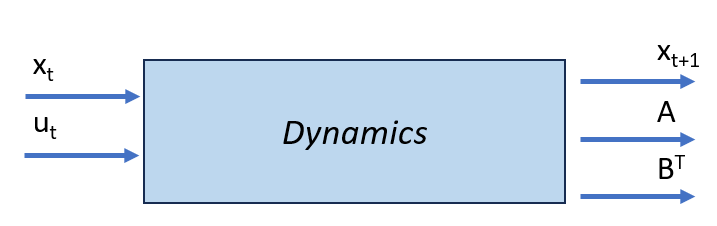
\includegraphics[width=0.5\textwidth]{pictures/dynamics.png}
\caption{\textit{Dynamics} function scheme block}
\label{fig:dynamics}
\end{figure}